\documentclass{beamer}

\usepackage{xcolor}
\usepackage{color}
\usepackage{hyperref}
\usepackage{wrapfig}

\usepackage{listings}

\graphicspath{{graphics/}}

\showboxdepth=\maxdimen
\showboxbreadth=\maxdimen

%~~~~~~~~~~~~~~~~~~~~~~~~~~~~~~~~~~~~~~~~~~~~~~~~~~~~~~~~~~~~~~~~~~~~~~~~~~~~~~
\definecolor{dkgreen}{rgb}{0.3,0.5,0.2}
\definecolor{gray}{rgb}{0.5,0.5,0.5}
\definecolor{mauve}{rgb}{0.58,0,0.82}
\definecolor{codepurple}{rgb}{0.58,0,0.82}

\lstset{basicstyle=\ttfamily,  
  showstringspaces=false,
  tab=\space\space\space,
  showtabs=true,
  commentstyle=\color{warning},
  keywordstyle=\color{white}
}
%~~~~~~~~~~~~~~~~~~~~~~~~~~~~~~~~~~~~~~~~~~~~~~~~~~~~~~~~~~~~~~~~~~~~~~~~~~~~~~

\title{Git Workshop}
\subtitle{Sobhan Ahmadian Moghadam}

\usetheme{lucid}

\begin{document}
	
	\frame {
		\titlepage
	}
	
	\frame{
		\frametitle{What is Git?}
		Git is a \textcolor{secondary}{free and open source}
		distributed version control
		system (\textcolor{secondary}{VCS}).
		
		\bigskip
		\noindent
		\textcolor{light-primary}{\href{https://git-scm.com}{Web page}}
	}
	
	\frame{
		\frametitle{What is VCS?}	
		
		\textcolor{secondary}{Control} of \textcolor{secondary}{code changes} over time.
	}
	
	\frame{
		\frametitle{What is VCS?}	
		
		What should we do if we want \textcolor{secondary}{manage} writing of a book:
		
		\begin{itemize}
			\item Save a few drafts
			\begin{itemize}
				\item \color{warning}{Waste storage}
				\item \color{warning}{The control is hard}
			\end{itemize}
			\item Use version control system
		\end{itemize}
	}
	
	\frame{
		\frametitle{What is Git?}
		Git is a \textcolor{secondary}{free and open source}
		distributed version control
		system (\textcolor{secondary}{VCS}).
		
		\begin{wrapfigure}{r}{4cm}
			\centering
			
\includegraphics[width=4cm]{git_logo}		
		\end{wrapfigure}		
		
		\noindent
		\begin{itemize}
			\item Version Control System
			\item Manage Code History
			\item Track Changes
		\end{itemize}
	}
	
	\frame{
		\frametitle{What is Github?}
		
		The largest and most advanced \textcolor{secondary}{development platform} in the world.
		
		\begin{wrapfigure}{r}{2.5cm}
			\centering
			
\includegraphics[width=2cm]{github}	
		\end{wrapfigure}
		
		\noindent
		\textcolor{light-primary}{\href{https://github.com/}{Web page}}
		
		\begin{itemize}
			\item Cloud Hosting
			\item Collaboration Provider
			\item \textcolor{secondary}{Git} Repository Hosting
		\end{itemize}
	}
	
	\frame{
		\frametitle{Command-line interface}
		
		A \textcolor{secondary}{text-based user interface} (UI) used to view and manage computer files.
		
		\noindent
		Users type \textcolor{secondary}{commands} in the command line interface to \textcolor{secondary}{run tasks} on a computer.
		
		\bigskip
		\begin{itemize}
			\item Windows : Command Prompt
			\item Linux : GNOME Terminal
		\end{itemize}

	}
	
	\frame{
		\frametitle{GNOME Terminal}
		\framesubtitle{commands}
		
		\begin{itemize}
			\item `\textbf{ls}' : list files
			\item `\textbf{cd}' : change directory
			\begin{itemize}
				\item `\textbf{cd ..}' back to upper directory
				\item `\textbf{cd [dir name]}' go to the directory
			\end{itemize}
			\item `\textbf{touch [file name]}' : make file
			\item `\textbf{rm [file name]}' : remove file
			\item `\textbf{mkdir [dir name]}' : make directory
			\item `\textbf{rmdir [dir name]}' : remove directory
		\end{itemize}
	}
	
	\frame{
		\frametitle{Command Prompt}
		\framesubtitle{commands}
		
		\begin{itemize}
			\item `\textbf{dir}' : list files
			\item `\textbf{cd}' : change directory
			\begin{itemize}
				\item `\textbf{cd ..}' back to upper directory
				\item `\textbf{cd [dir name]}' go to the directory
			\end{itemize}
			\item `\textbf{cls}' : clean cmd
			\item `\textbf{mkdir [dir name]}' : make directory
			\item `\textbf{rmdir [dir name]}' : remove directory
			\item `\textbf{echo [content] > [file name]}' : make file
			\item `\textbf{del [file name]}' : delete file
		\end{itemize}
	}
	
	\begin{frame}[fragile]
		\frametitle{Install Git}
		\framesubtitle{Linux}
		
		\begin{itemize}
			\item \textcolor{light-primary}{\href{https://git-scm.com}{Web page}}
			> Downloads > Linux/Unix
			\item
\begin{lstlisting}[language=bash]
$ sudo apt-get install git
\end{lstlisting}		
		\end{itemize}
	
	\end{frame}
	
	\begin{frame}[fragile]
		\frametitle{Git Version}	
		\framesubtitle{Linux}	

\begin{lstlisting}[language=bash]
$ git --version
\end{lstlisting}	

	\end{frame}
	
	\begin{frame}[fragile]
		\frametitle{Update Git}
		\framesubtitle{Linux}
		
\begin{lstlisting}[language=bash]
$ sudo add-apt-repository -y ppa:git-core/ppa
$ sudo apt-get update
$ sudo apt-get install git -y
\end{lstlisting}		

	\end{frame}
	
	\begin{frame}
		\frametitle{Install Git}
		\framesubtitle{Windows}
		\begin{itemize}
			\item \textcolor{light-primary}{\href{https://git-scm.com}{Web page}}
			> Downloads > Windows
			\item Run .exe file
			\item Leave settings by default
		\end{itemize}
	\end{frame}

	\begin{frame}[fragile]
		\frametitle{Git Version}
		\framesubtitle{Windows}
\begin{lstlisting}[language=bash]
$ git --version
\end{lstlisting}
	\end{frame}
		
	\begin{frame}[fragile]
		\frametitle{Install Git}
		\framesubtitle{macOS}
		
		\begin{itemize}
			\item \textcolor{light-primary}{\href{https://git-scm.com}{Web page}}
			> Downloads > macOS
			\item install \textcolor{light-primary}{\href{https://brew.sh}{Homebrew}}
			\item
\begin{lstlisting}[language=bash]
$ brew install git
\end{lstlisting}
		\end{itemize}
	\end{frame}
	
	\begin{frame}[fragile]
		\frametitle{Git Version}
		\framesubtitle{macOS}
\begin{lstlisting}[language=bash]
$ git --version
\end{lstlisting}
	\end{frame}
	
	\frame{
		\frametitle{How Git Works?}
		\framesubtitle{abstract example}
		
		\begin{figure}[htbp]
			\centering
			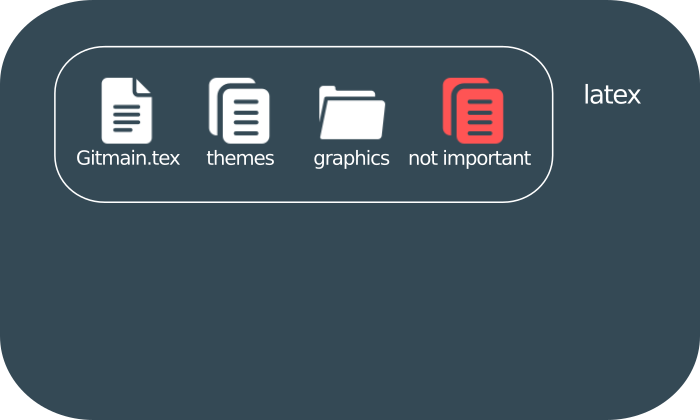
\includegraphics[width=10cm]{howgitwork1}
		\end{figure}
	}
	
	\frame{
		\frametitle{How Git Works?}
		\framesubtitle{abstract example}
		
		\begin{figure}[htbp]
			\centering
			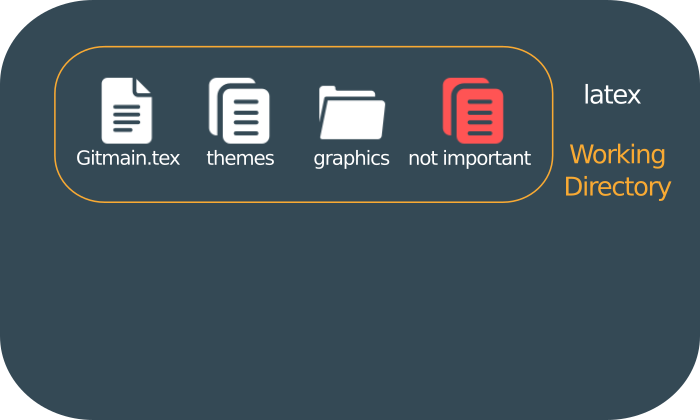
\includegraphics[width=10cm]{howgitwork2}
		\end{figure}
	}
	
	\frame{
		\frametitle{How Git Works?}
		\framesubtitle{abstract example}
		
		\begin{figure}[htbp]
			\centering
			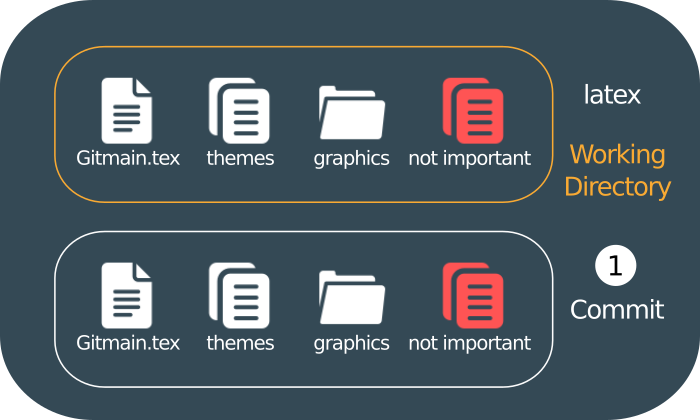
\includegraphics[width=10cm]{howgitwork3}
		\end{figure}
	}
	
	\frame{
		\frametitle{How Git Works?}
		\framesubtitle{abstract example}
		
		\begin{figure}[htbp]
			\centering
			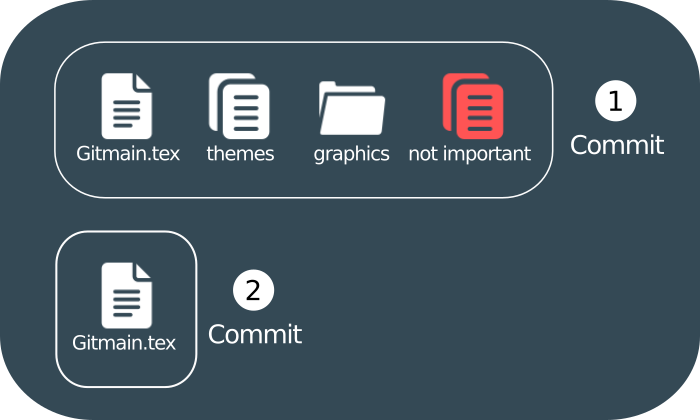
\includegraphics[width=10cm]{howgitwork4}
		\end{figure}
	}
	
	\frame{
		\frametitle{How Git Works?}
		\framesubtitle{abstract example}
		
		\begin{figure}[htbp]
			\centering
			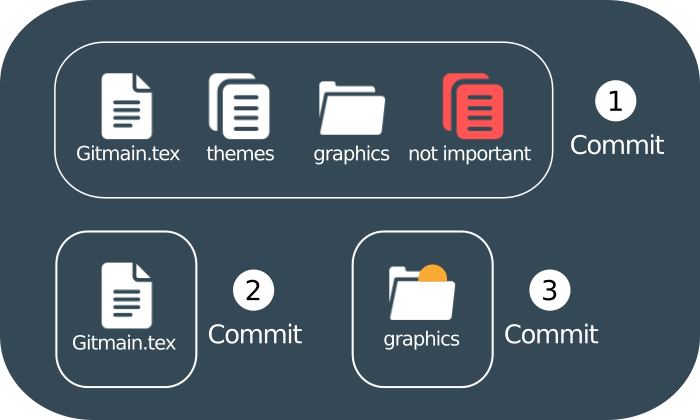
\includegraphics[width=10cm]{howgitwork5}
		\end{figure}
	}

	\frame{
		\frametitle{How Git Works?}
		\framesubtitle{abstract example}
		
		\begin{figure}[htbp]
			\centering
			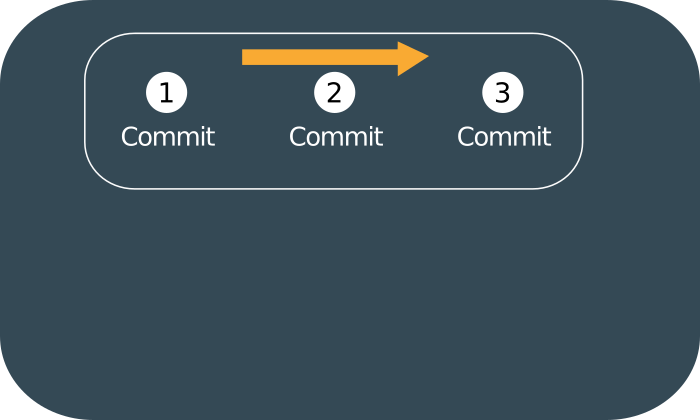
\includegraphics[width=10cm]{howgitwork6}
		\end{figure}
	}
	
	\frame{
		\frametitle{How Git Works?}
		\framesubtitle{abstract example}
		
		\begin{figure}[htbp]
			\centering
			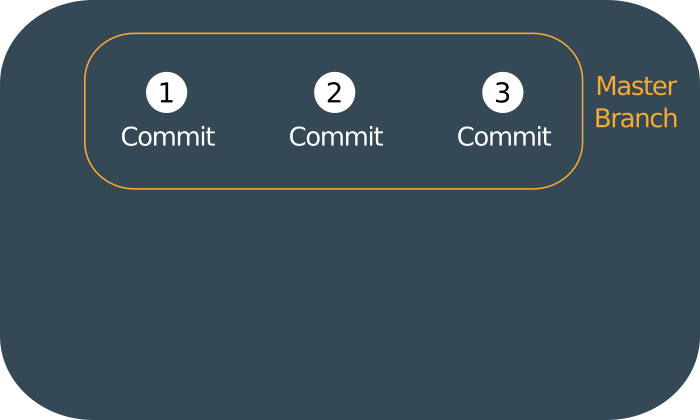
\includegraphics[width=10cm]{howgitwork7}
		\end{figure}
	}
	
	\frame{
		\frametitle{How Git Works?}
		\framesubtitle{abstract example}
		
		\begin{figure}[htbp]
			\centering
			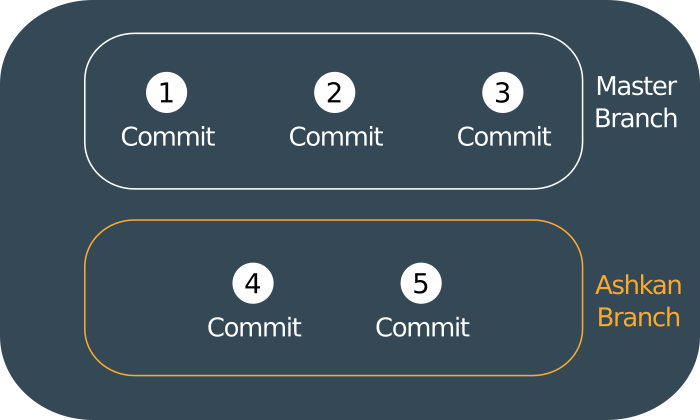
\includegraphics[width=10cm]{howgitwork8}
		\end{figure}
	}
	
	\frame{
		\frametitle{How Git Works?}
		\framesubtitle{abstract example}
		
		\begin{figure}[htbp]
			\centering
			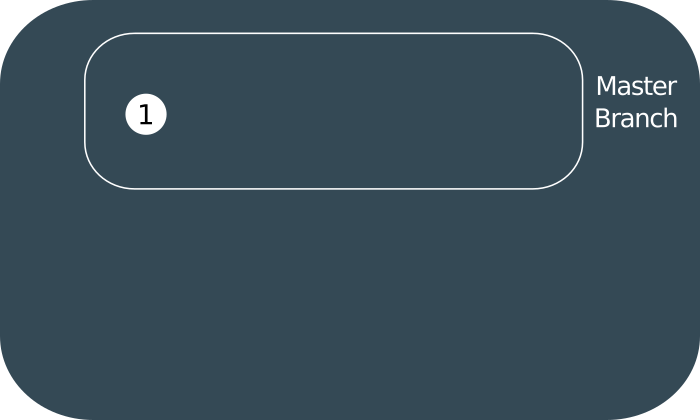
\includegraphics[width=10cm]{howgitwork9}
		\end{figure}
	}
	
	\frame{
		\frametitle{How Git Works?}
		\framesubtitle{abstract example}
		
		\begin{figure}[htbp]
			\centering
			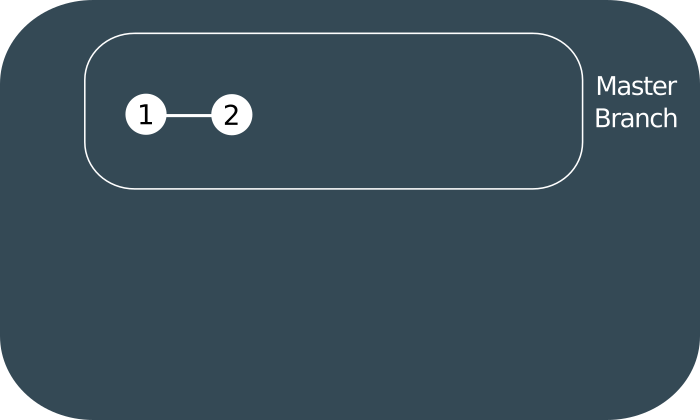
\includegraphics[width=10cm]{howgitwork10}
		\end{figure}
	}
	
	\frame{
		\frametitle{How Git Works?}
		\framesubtitle{abstract example}
		
		\begin{figure}[htbp]
			\centering
			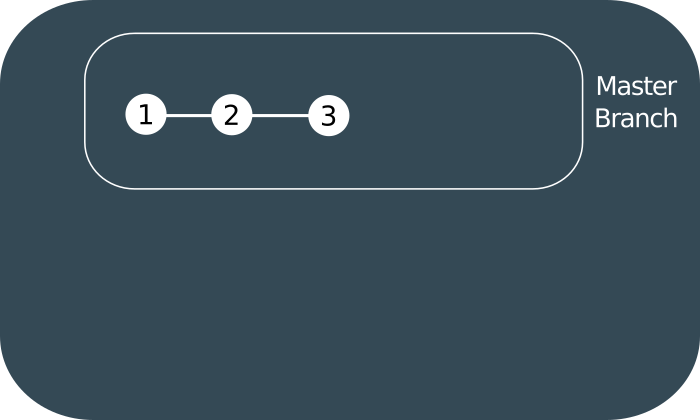
\includegraphics[width=10cm]{howgitwork11}
		\end{figure}
	}
	
	\frame{
		\frametitle{How Git Works?}
		\framesubtitle{abstract example}
		
		\begin{figure}[htbp]
			\centering
			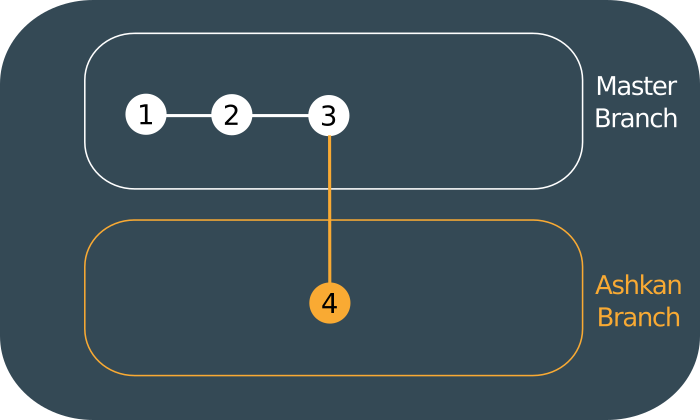
\includegraphics[width=10cm]{howgitwork12}
		\end{figure}
	}
	
	\frame{
		\frametitle{How Git Works?}
		\framesubtitle{abstract example}
		
		\begin{figure}[htbp]
			\centering
			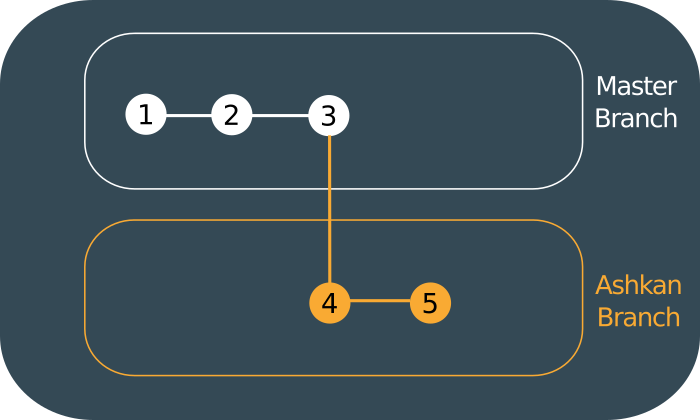
\includegraphics[width=10cm]{howgitwork13}
		\end{figure}
	}
	
	\frame{
		\frametitle{How Git Works?}
		\framesubtitle{abstract example}
		
		\begin{figure}[htbp]
			\centering
			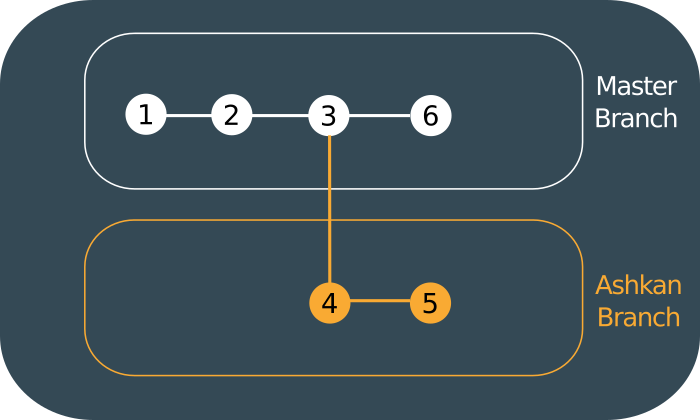
\includegraphics[width=10cm]{howgitwork14}
		\end{figure}
	}
	
	\frame{
		\frametitle{How Git Works?}
		\framesubtitle{abstract example}
		
		\begin{figure}[htbp]
			\centering
			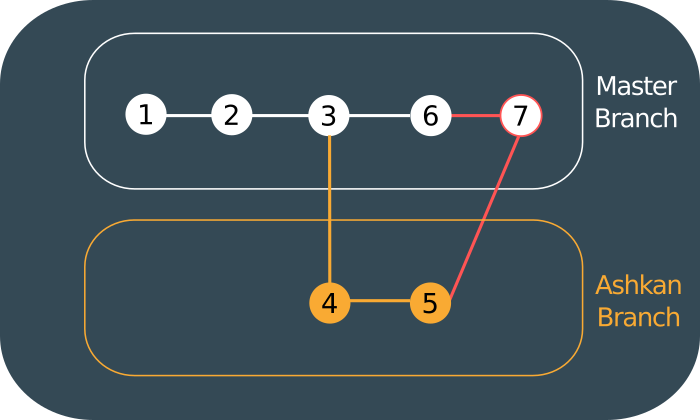
\includegraphics[width=10cm]{howgitwork15}
		\end{figure}
	}
		
	\begin{frame}[fragile]
		\frametitle{Git Commands}
		\framesubtitle{status and initial}

First check that git is installed.\\
Then check git status.\\
If there is no git repository, initial git.

\begin{lstlisting}[language=bash]
# get git version
$ git --version

# get git status
$ git status

# initial git for current repository
$ git init
\end{lstlisting}

	\end{frame}
	
	\begin{frame}[fragile]
		\frametitle{Git Commands}
		\framesubtitle{configuration}
		
		Set email and username (If you didn't do that before).		
		
\begin{lstlisting}[language=bash]
# show git configuration
$ git config --list

# set email and username
$ git config --global user.email "<email>"
$ git config --global user.name "<Your Name>"

# unset email and username
$ git config --global --unset user.name
$ git config --global --unset user.email
\end{lstlisting}
	
	\end{frame}
	
	\begin{frame}
		\frametitle{Staging}
		\begin{figure}[htbp]
			\centering
			
\includegraphics[width=10cm]{staging1}
		\end{figure}
	\end{frame}
	
	\begin{frame}
		\frametitle{Staging}
		\begin{figure}[htbp]
			\centering
			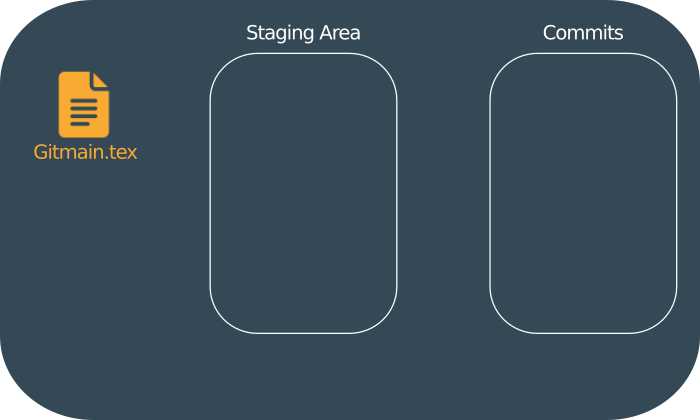
\includegraphics[width=10cm]{staging2}
		\end{figure}
	\end{frame}
	
	\begin{frame}
		\frametitle{Staging}
		\begin{figure}[htbp]
			\centering
			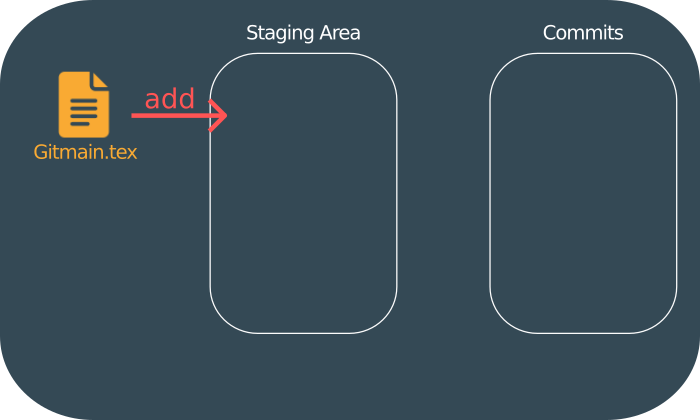
\includegraphics[width=10cm]{staging3}
		\end{figure}
	\end{frame}
	
	\begin{frame}
		\frametitle{Staging}
		\begin{figure}[htbp]
			\centering
			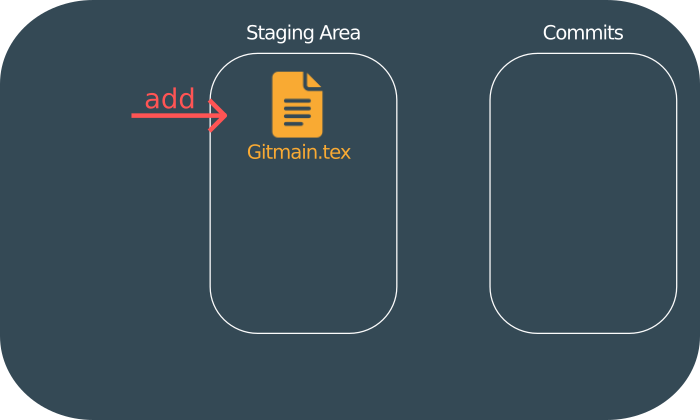
\includegraphics[width=10cm]{staging4}
		\end{figure}
	\end{frame}
	
	\begin{frame}
		\frametitle{Staging}
		\begin{figure}[htbp]
			\centering
			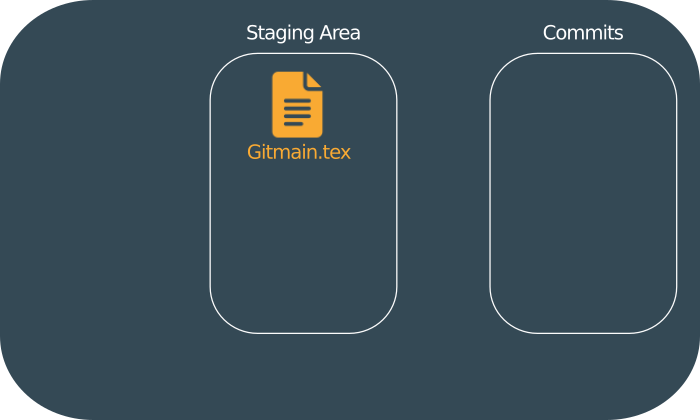
\includegraphics[width=10cm]{staging5}
		\end{figure}
	\end{frame}
	
	\begin{frame}
		\frametitle{Staging}
		\begin{figure}[htbp]
			\centering
			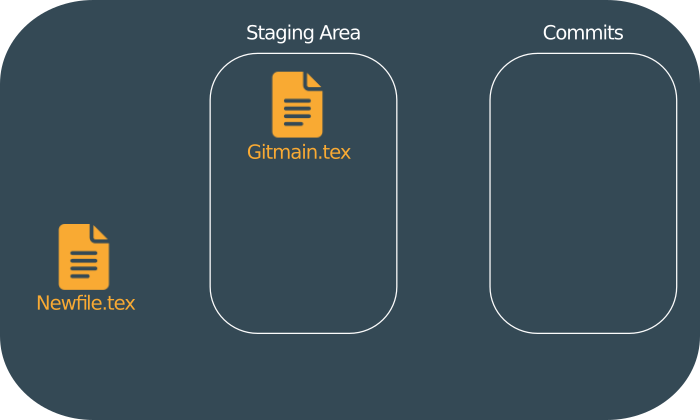
\includegraphics[width=10cm]{staging6}
		\end{figure}
	\end{frame}
	
	\begin{frame}
		\frametitle{Staging}
		\begin{figure}[htbp]
			\centering
			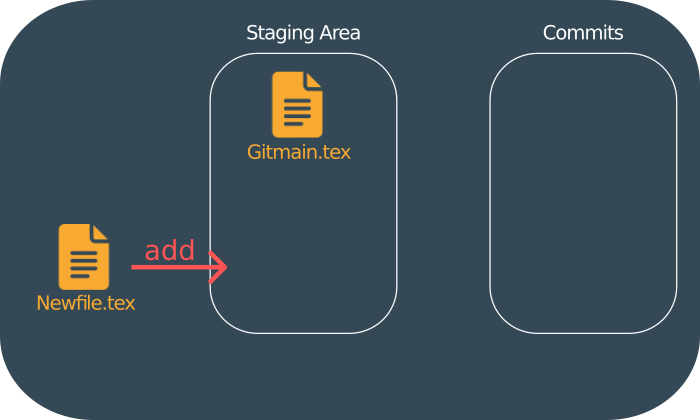
\includegraphics[width=10cm]{staging7}
		\end{figure}
	\end{frame}
	
	\begin{frame}
		\frametitle{Staging}
		\begin{figure}[htbp]
			\centering
			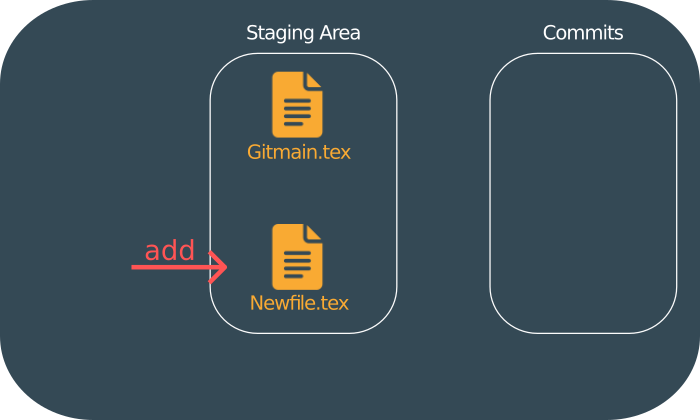
\includegraphics[width=10cm]{staging8}
		\end{figure}
	\end{frame}
	
	\begin{frame}
		\frametitle{Staging}
		\begin{figure}[htbp]
			\centering
			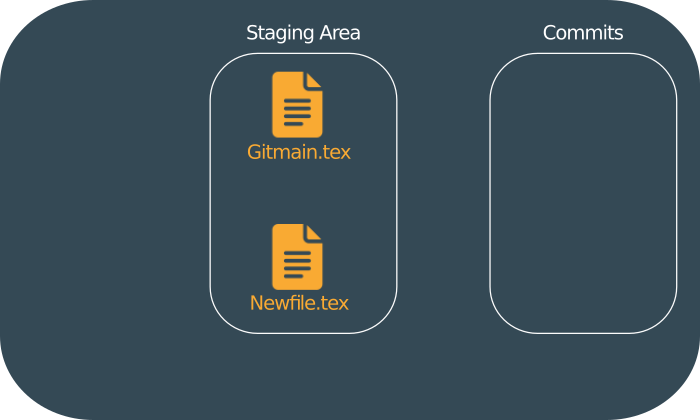
\includegraphics[width=10cm]{staging9}
		\end{figure}
	\end{frame}
	
	\begin{frame}
		\frametitle{Staging}
		\begin{figure}[htbp]
			\centering
			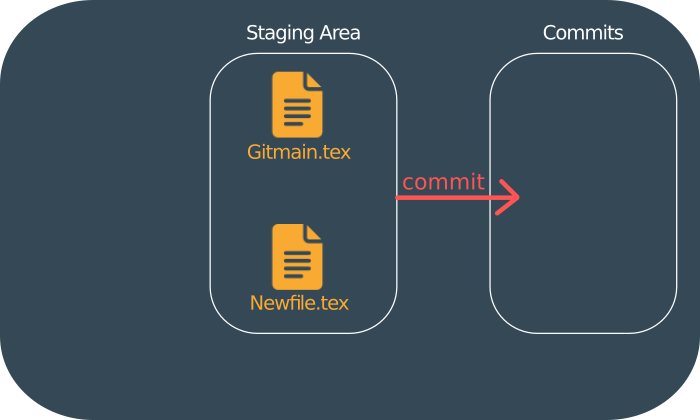
\includegraphics[width=10cm]{staging10}
		\end{figure}
	\end{frame}
	
	\begin{frame}
		\frametitle{Staging}
		\begin{figure}[htbp]
			\centering
			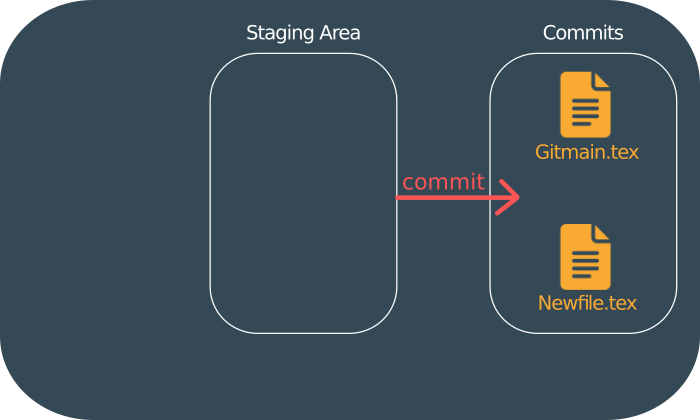
\includegraphics[width=10cm]{staging11}
		\end{figure}
	\end{frame}
	
	\begin{frame}
		\frametitle{Staging}
		\begin{figure}[htbp]
			\centering
			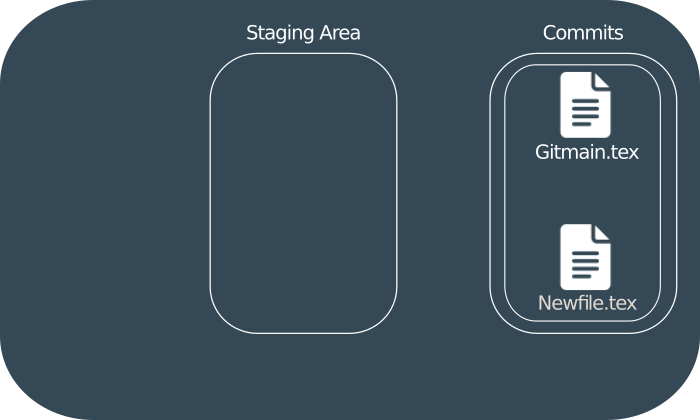
\includegraphics[width=10cm]{staging12}
		\end{figure}
	\end{frame}
	
	\begin{frame}[fragile]
		\frametitle{Git Commands}
		\framesubtitle{stage and commit}	
		
\begin{lstlisting}[language=bash]
# add file to staging area
$ git add <file name>

# add all changes to staging area
$ git add .

# remove file from staging area
$ git restore --staged <file name>

# commit changes
$ git commit -m "<message>"
\end{lstlisting}
	
	\end{frame}
	
	\begin{frame}[fragile]
		\frametitle{Git Commands}
		\framesubtitle{switch to a commit}	
		
\begin{lstlisting}[language=bash]
# show commits in current branch
$ git log

# switch to a commit
$ git checkout <commit id>
\end{lstlisting}
	
	\end{frame}
	
	\begin{frame}[fragile]
		\frametitle{Git Commands}
		\framesubtitle{branches}	
		
\begin{lstlisting}[language=bash]
# show branches
$ git branch

# create a new branch
$ git branch <branch name>

# switch to a branch
$ git checkout <branch name>

# shortcut for create and move to a branch
$ git checkout -b <branch name>
\end{lstlisting}
	
	\end{frame}

	\begin{frame}[fragile]
		\frametitle{Git Commands}
		\framesubtitle{merge branches}	
		
\begin{lstlisting}[language=bash]
# merge a branch to current branch
$ git merge <branch name>
\end{lstlisting}
	
	\end{frame}
	
	\begin{frame}
		\frametitle{Head}
		\begin{figure}[htbp]
			\centering
			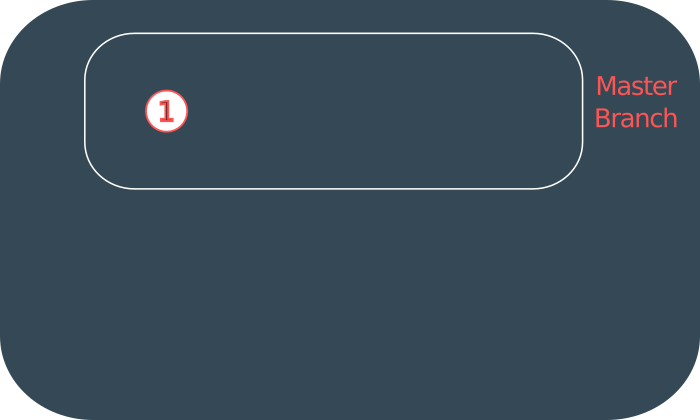
\includegraphics[width=10cm]{head1}
		\end{figure}
	\end{frame}
	
	\begin{frame}
		\frametitle{Head}
		\begin{figure}[htbp]
			\centering
			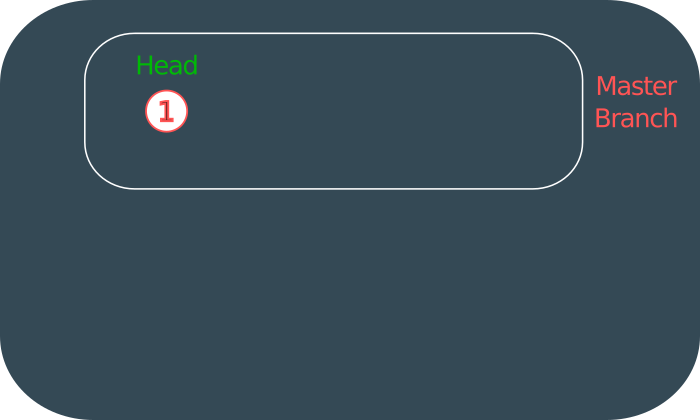
\includegraphics[width=10cm]{head2}
		\end{figure}
	\end{frame}
	
	\begin{frame}
		\frametitle{Head}
		\begin{figure}[htbp]
			\centering
			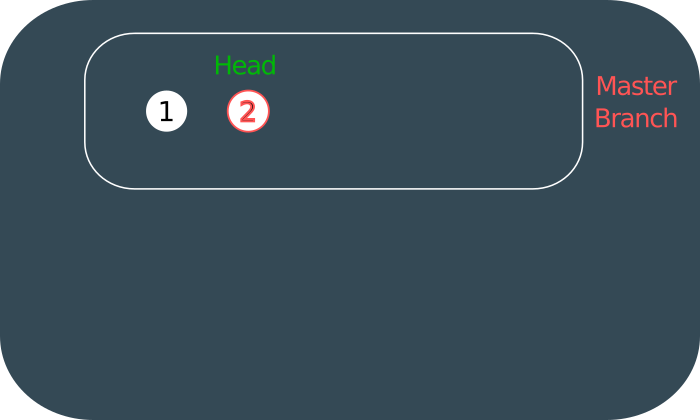
\includegraphics[width=10cm]{head3}
		\end{figure}
	\end{frame}
	
	\begin{frame}
		\frametitle{Head}
		\begin{figure}[htbp]
			\centering
			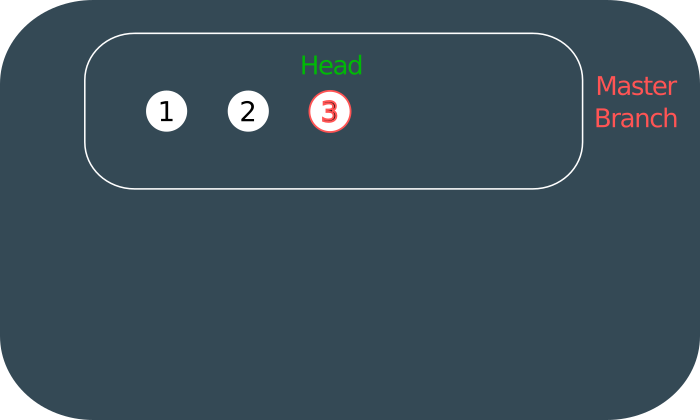
\includegraphics[width=10cm]{head4}
		\end{figure}
	\end{frame}
	
	\begin{frame}
		\frametitle{Head}
		\begin{figure}[htbp]
			\centering
			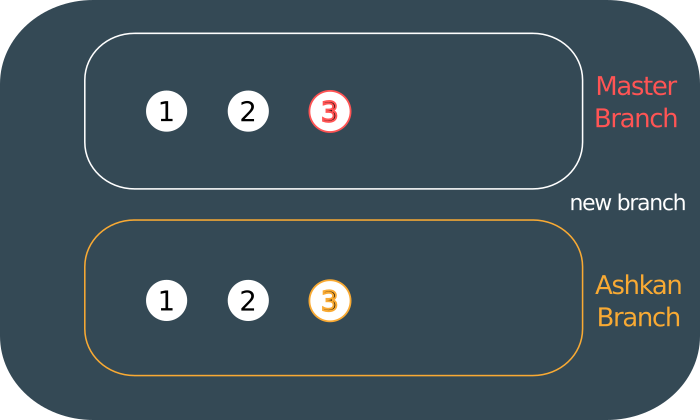
\includegraphics[width=10cm]{head5}
		\end{figure}
	\end{frame}
	
	\begin{frame}
		\frametitle{Head}
		\begin{figure}[htbp]
			\centering
			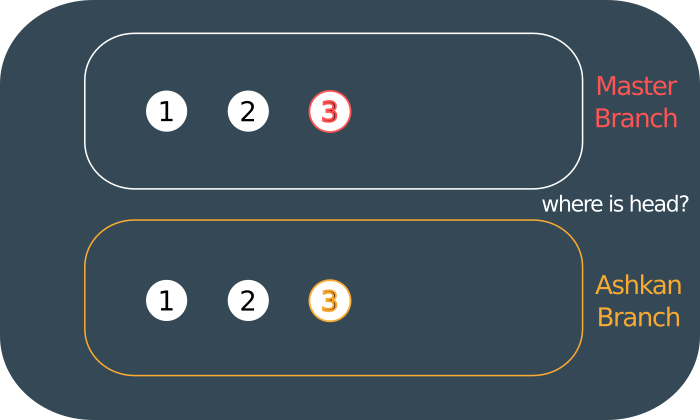
\includegraphics[width=10cm]{head6}
		\end{figure}
	\end{frame}
	
	\begin{frame}
		\frametitle{Head}
		\begin{figure}[htbp]
			\centering
			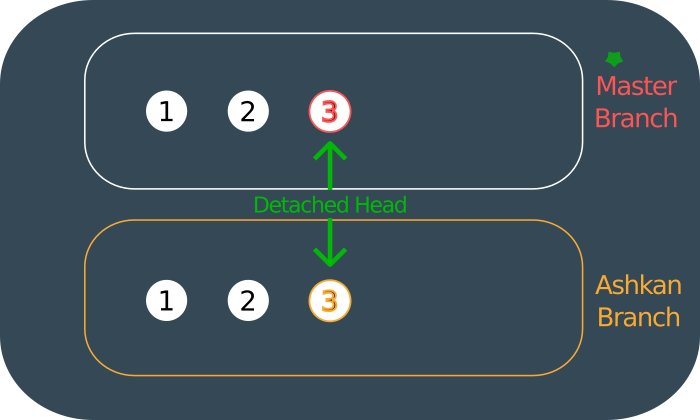
\includegraphics[width=10cm]{head7}
		\end{figure}
	\end{frame}
	
	\begin{frame}
		\frametitle{Head}
		\begin{figure}[htbp]
			\centering
			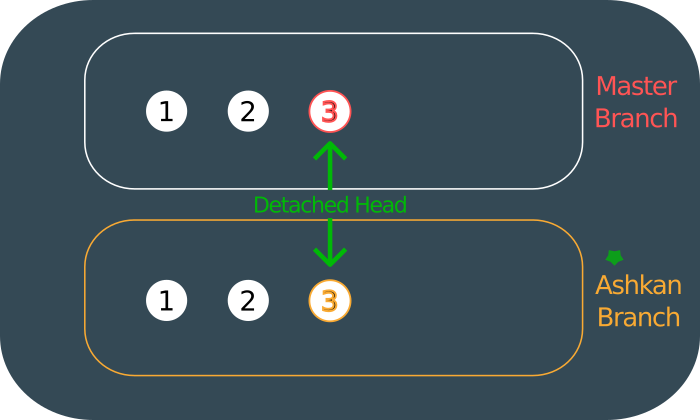
\includegraphics[width=10cm]{head8}
		\end{figure}
	\end{frame}
	
	\begin{frame}
		\frametitle{Head}
		\begin{figure}[htbp]
			\centering
			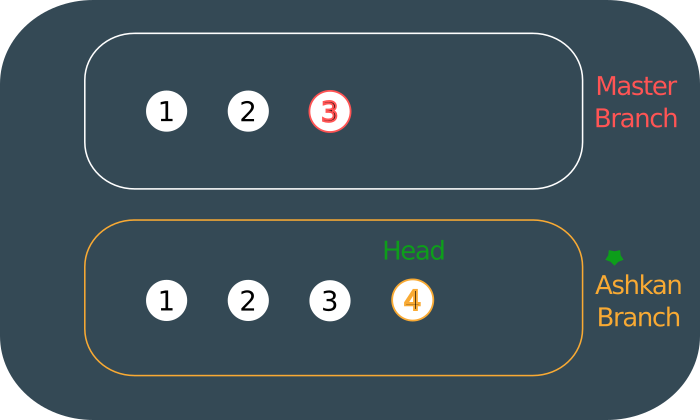
\includegraphics[width=10cm]{head9}
		\end{figure}
	\end{frame}
	
	\begin{frame}
		\frametitle{Head}
		\begin{figure}[htbp]
			\centering
			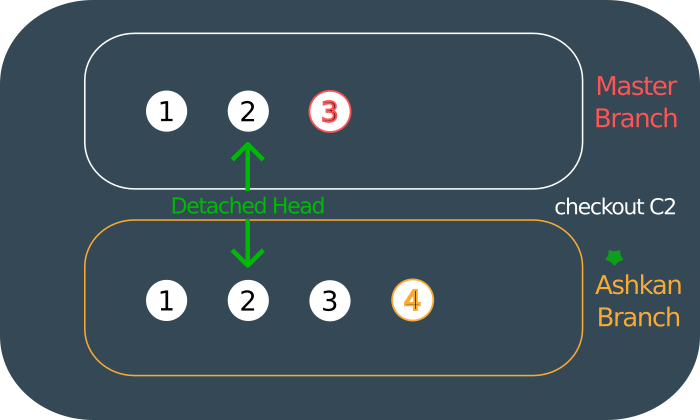
\includegraphics[width=10cm]{head10}
		\end{figure}
	\end{frame}
	
	\begin{frame}
		\frametitle{Head}
		\begin{figure}[htbp]
			\centering
			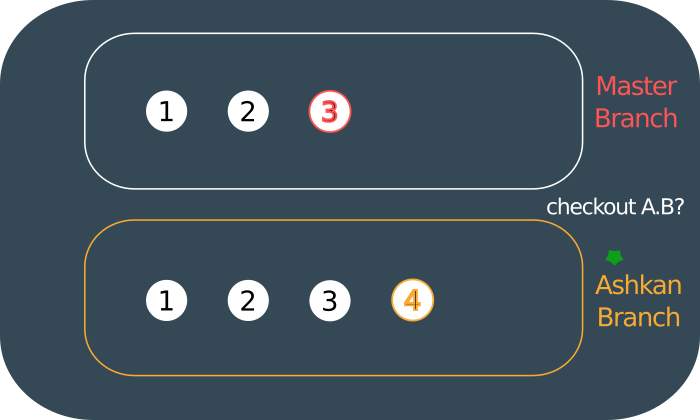
\includegraphics[width=10cm]{head11}
		\end{figure}
	\end{frame}
	
	\begin{frame}
		\frametitle{Head}
		\begin{figure}[htbp]
			\centering
			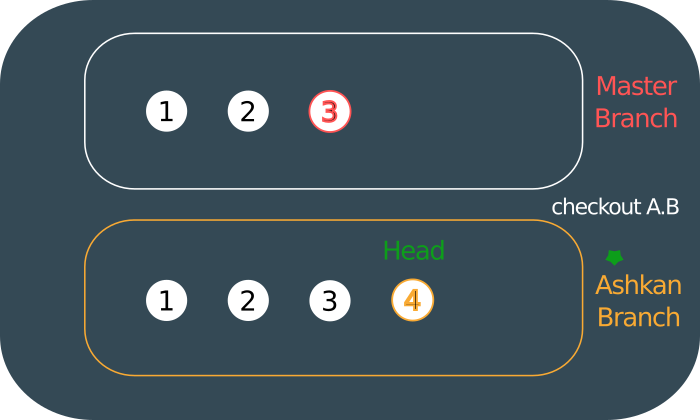
\includegraphics[width=10cm]{head12}
		\end{figure}
	\end{frame}
	
	\begin{frame}
		\frametitle{Head}
		\begin{figure}[htbp]
			\centering
			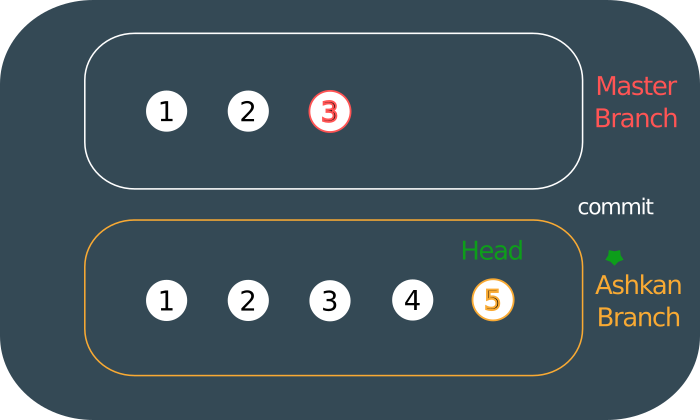
\includegraphics[width=10cm]{head13}
		\end{figure}
	\end{frame}
	
	\begin{frame}
		\frametitle{Head}
		\begin{figure}[htbp]
			\centering
			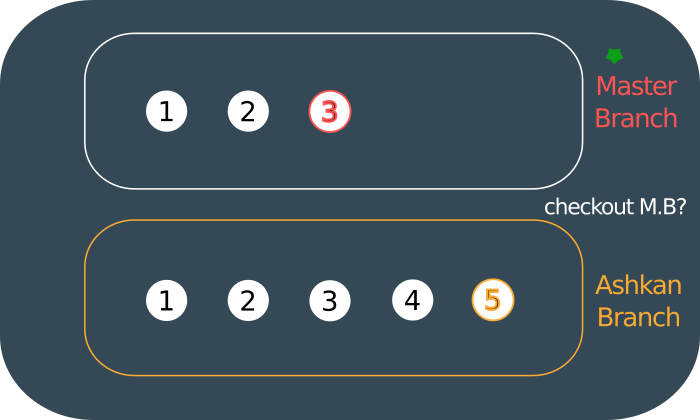
\includegraphics[width=10cm]{head14}
		\end{figure}
	\end{frame}
	
	\begin{frame}
		\frametitle{Head}
		\begin{figure}[htbp]
			\centering
			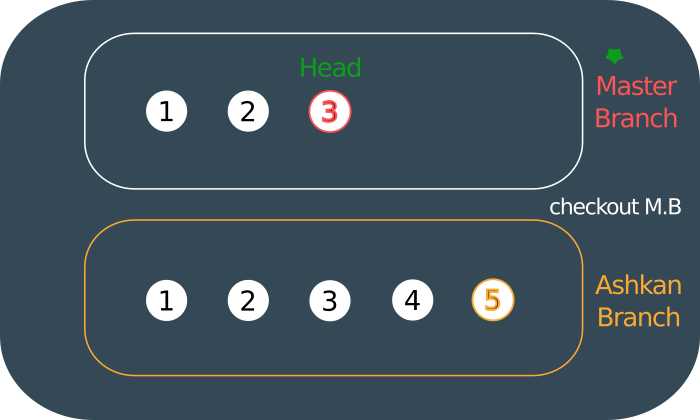
\includegraphics[width=10cm]{head15}
		\end{figure}
	\end{frame}
	
	\begin{frame}
		\frametitle{Head}
		\begin{figure}[htbp]
			\centering
			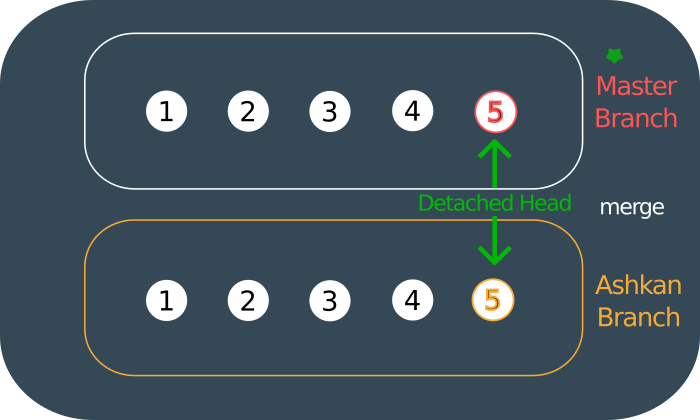
\includegraphics[width=10cm]{head16}
		\end{figure}
	\end{frame}
	
	\begin{frame}
		\frametitle{Deleting Data}
		\begin{itemize}
			\item Working Directory Files
			\item Unstaged Changes
			\item Staged Changes
			\item Latest Commit(s)
			\item Branches
		\end{itemize}
	\end{frame}
	
	\begin{frame}[fragile]
		\frametitle{Deleting Data}
		\framesubtitle{Working Directory Files}
		
		\begin{itemize}
			\item Move the file from working directory to trash
			\item 
\begin{lstlisting}[language=bash]
$ git rm <file name>
\end{lstlisting}
			\item commit
		\end{itemize}
	\end{frame}
	
	\begin{frame}[fragile]
		\frametitle{Deleting Data}
		\framesubtitle{Unstaged Changes}
		
\begin{lstlisting}[language=bash]
# remove unstaged changes in a file
$ git checkout <filename>
# or
$ git restore <filename>

# remove unstaged changes in all files
$ git checkout .
# or
$ git restore .
\end{lstlisting}
	\end{frame}

	\begin{frame}[fragile]
		\frametitle{Deleting Data}
		\framesubtitle{Unstaged Changes}
		
\begin{lstlisting}[language=bash]
# remove untracked file

# first check what will be removed
$ git clean -dn

# then force delete that
$ git chean -df
\end{lstlisting}
	\end{frame}
	
	\begin{frame}[fragile]
		\frametitle{Deleting Data}
		\framesubtitle{Staged Changes}
		
\begin{lstlisting}[language=bash]
# unstage staged file
$ git restore --staged <file name>

# delete unstaged change
$ git restore <file name>
\end{lstlisting}
	\end{frame}

	\begin{frame}[fragile]
		\frametitle{Deleting Data}
		\framesubtitle{Latest Commit(s)}
		
\begin{lstlisting}[language=bash]
# keep new files staged
$ git reset --soft HEAD~1

# keep new files unstaged
$ git reset HEAD~1

# remove new files
$ git reset --hard HEAD~1
\end{lstlisting}
	\end{frame}

	\begin{frame}[fragile]
		\frametitle{Deleting Data}
		\framesubtitle{Branches}
		
\begin{lstlisting}[language=bash]
$ git branch -D <branch name>
\end{lstlisting}
	\end{frame}
	
	\begin{frame}
		\frametitle{Gitignore}
		
		.gitignore file contains file that you don't want to track in git management.\\
		you should create it in work directory.\\
		each line one record.
		
		\begin{itemize}
			\item `<filename>' ignores file
			\item `*.<extension>' ignore all files with a extension
			\item `!<file name>' remove file from being ignored
			\item `<dir>/*' ignores all files in directory
		\end{itemize}
		
		check this \textcolor{light-primary}{\href{https://github.com/github/gitignore}{Web page}} for some gitignore files.
	\end{frame}
	
	\begin{frame}[fragile]
		\frametitle{Restore Data}
		
\begin{lstlisting}[language=bash]
# check logs by following command
$ git reflog

# moving head to a commit
$ git checkout <commit>

# moving branch pointer to a commit
$ git branch -f <branch-name> <sha1-commit-hash>
\end{lstlisting}
	\end{frame}
	
	\begin{frame}
		\frametitle{Fast Forward Merge}
		\begin{figure}[htbp]
			\centering
			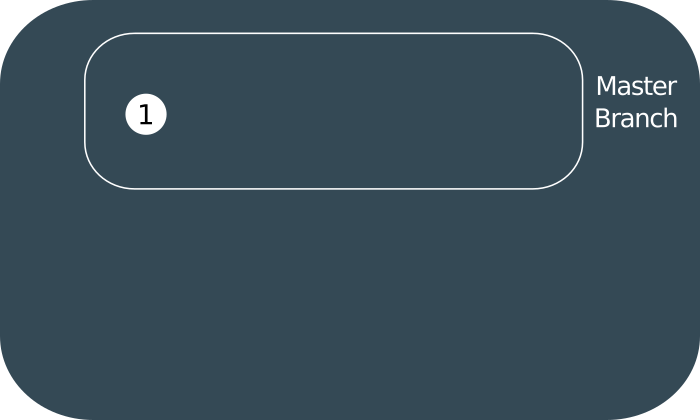
\includegraphics[width=10cm]{howgitwork9}
		\end{figure}
	\end{frame}
	
	\begin{frame}
		\frametitle{Fast Forward Merge}
		\begin{figure}[htbp]
			\centering
			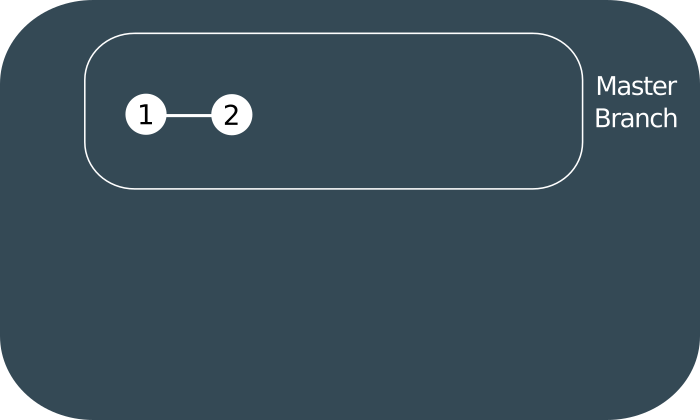
\includegraphics[width=10cm]{howgitwork10}
		\end{figure}
	\end{frame}
	
	\begin{frame}
		\frametitle{Fast Forward Merge}
		\begin{figure}[htbp]
			\centering
			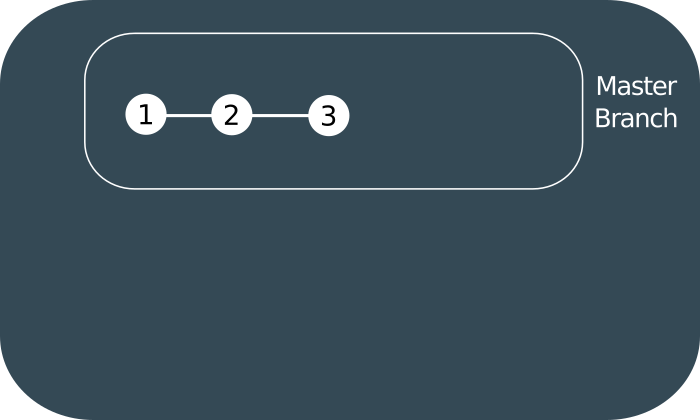
\includegraphics[width=10cm]{howgitwork11}
		\end{figure}
	\end{frame}
	
	\begin{frame}
		\frametitle{Fast Forward Merge}
		\begin{figure}[htbp]
			\centering
			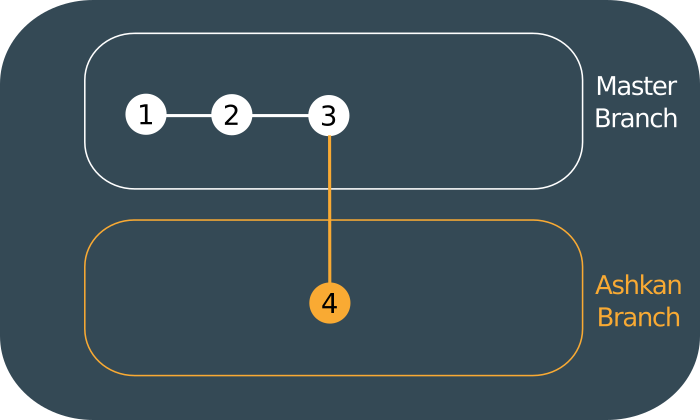
\includegraphics[width=10cm]{howgitwork12}
		\end{figure}
	\end{frame}
	
	\begin{frame}
		\frametitle{Fast Forward Merge}
		\begin{figure}[htbp]
			\centering
			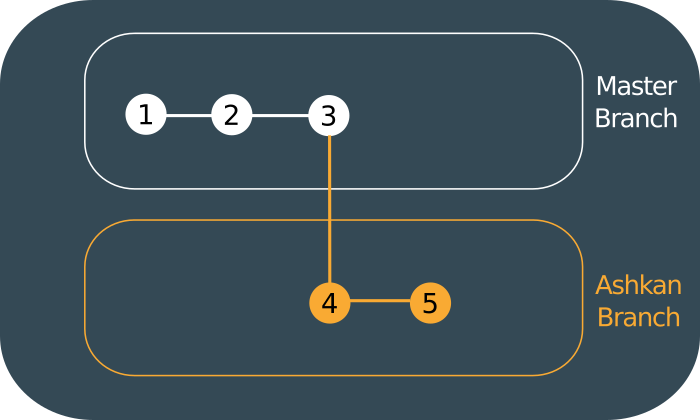
\includegraphics[width=10cm]{howgitwork13}
		\end{figure}
	\end{frame}
	
	\begin{frame}
		\frametitle{Fast Forward Merge}
		\begin{figure}[htbp]
			\centering
			\includegraphics[width=10cm]{fastforwardmerge1}
		\end{figure}
	\end{frame}
	
	\begin{frame}
		\frametitle{Merge}
		\begin{figure}[htbp]
			\centering
			\includegraphics[width=10cm]{howgitwork9}
		\end{figure}
	\end{frame}
	
	\begin{frame}
		\frametitle{Merge}
		\begin{figure}[htbp]
			\centering
			\includegraphics[width=10cm]{howgitwork10}
		\end{figure}
	\end{frame}
	
	\begin{frame}
		\frametitle{Merge}
		\begin{figure}[htbp]
			\centering
			\includegraphics[width=10cm]{howgitwork11}
		\end{figure}
	\end{frame}
	
	\begin{frame}
		\frametitle{Merge}
		\begin{figure}[htbp]
			\centering
			\includegraphics[width=10cm]{howgitwork12}
		\end{figure}
	\end{frame}
	
	\begin{frame}
		\frametitle{Merge}
		\begin{figure}[htbp]
			\centering
			\includegraphics[width=10cm]{howgitwork13}
		\end{figure}
	\end{frame}
	
	\begin{frame}
		\frametitle{Merge}
		\begin{figure}[htbp]
			\centering
			\includegraphics[width=10cm]{howgitwork14}
		\end{figure}
	\end{frame}
	
	\begin{frame}
		\frametitle{Merge}
		\begin{figure}[htbp]
			\centering
			\includegraphics[width=10cm]{howgitwork15}
		\end{figure}
	\end{frame}

	\begin{frame}
		\frametitle{Github and Git}
		\begin{figure}[htbp]
			\centering
			\includegraphics[width=10cm]{githubgit1}
		\end{figure}
	\end{frame}
	
	\begin{frame}
		\frametitle{Github and Git}
		\begin{figure}[htbp]
			\centering
			\includegraphics[width=10cm]{githubgit2}
		\end{figure}
	\end{frame}
	
	\begin{frame}
		\frametitle{Github and Git}
		\begin{figure}[htbp]
			\centering
			\includegraphics[width=10cm]{githubgit3}
		\end{figure}
	\end{frame}
	
	\begin{frame}[fragile]
		\frametitle{Github and Git}
		\begin{itemize}
			\item push your local repository to remote repository
			\item 
\begin{lstlisting}[language=bash]
# show local branches
$ git branch

# show local and remote branches
$ git branch -a
\end{lstlisting}		
		\end{itemize}
	\end{frame}
	
	\begin{frame}
		\frametitle{Warning}
		in upcoming slides instead of local tracking branch should be remote tracking branch
	\end{frame}		
	
	\begin{frame}
		\frametitle{Github and Git}
		\framesubtitle{branches}
		\begin{figure}[htbp]
			\centering
			\includegraphics[width=10cm]{remotebranch1}
		\end{figure}
	\end{frame}
	
	\begin{frame}
		\frametitle{Github and Git}
		\framesubtitle{branches}
		\begin{figure}[htbp]
			\centering
			\includegraphics[width=10cm]{remotebranch2}
		\end{figure}
	\end{frame}
	
	\begin{frame}
		\frametitle{Github and Git}
		\framesubtitle{branches}
		\begin{figure}[htbp]
			\centering
			\includegraphics[width=10cm]{remotebranch3}
		\end{figure}
	\end{frame}
	
	\begin{frame}
		\frametitle{Github and Git}
		\framesubtitle{branches}
		\begin{figure}[htbp]
			\centering
			\includegraphics[width=10cm]{remotebranch4}
		\end{figure}
	\end{frame}
	
	\begin{frame}
		\frametitle{Github and Git}
		\framesubtitle{branches}
		\begin{figure}[htbp]
			\centering
			\includegraphics[width=10cm]{remotebranch5}
		\end{figure}
	\end{frame}
	
	\begin{frame}
		\frametitle{Github and Git}
		\framesubtitle{branches}
		\begin{figure}[htbp]
			\centering
			\includegraphics[width=10cm]{remotebranch7}
		\end{figure}
	\end{frame}
	
	\begin{frame}
		\frametitle{Github and Git}
		\framesubtitle{branches}
		\begin{figure}[htbp]
			\centering
			\includegraphics[width=10cm]{remotebranch8}
		\end{figure}
	\end{frame}

	\begin{frame}[fragile]
		\frametitle{Github and Git}
		\framesubtitle{add branch to remote repository}
\begin{lstlisting}[language=bash]
# show remote branches
$ git ls-remote

# sync remote branch and its local tracking branch
$ git fetch

# fast forward merge
$ merge <local tracking branch>

# fetch and merge
$ git pull <remote> <branch>
\end{lstlisting}		
	\end{frame}
	
	\begin{frame}
		\frametitle{Branch type}
		\begin{itemize}
			\item local branch
			\item remote branch
			\item remote tracking branch
		\end{itemize}
	\end{frame}

	\begin{frame}
		\frametitle{Branch type}
		\begin{itemize}
			\item local branch
			\item remote branch
			\item remote tracking branch
			\item local tracking branch		
		\end{itemize}
	\end{frame}

	\begin{frame}[fragile]
		\frametitle{Branch type}
		\framesubtitle{local tracking branch}
		Local reference to remote tracking branch

\begin{lstlisting}[language=bash]
$ git push -u origing <branch>

# create a local tracking branch
$ git branch --track <name> <remote.t.b>

# show type of branches
$ git branch -vv
\end{lstlisting}	
		
	\end{frame}

\end{document}